\section{Experiments} \label{sec:experiment}
In this section, we measure the overall performance of the optimized 
HLS based BFS accelerator on Alpha Data ADM-PCIE-7v3 using a set of 
representative graphs and compare it to both a baseline design 
and existing FPGA based BFS acceleration work. Then we evaluate the major design 
optimization methods including pipelining, redundancy removal,  
caching and data path duplication with an incremental manner. 
For each optimization method, the design trade-offs are discussed with 
comprehensive experiments. 

\subsection{Experiment Setup}
The graph benchmark used in this work includes three real-world graphs and two graphs 
generated using R-MAT model \cite{chakrabarti2004rmat} as listed in 
Table \ref{tab:graph}. The real-world graphs are from social network \cite{yang2012defining, 
leskovec2009community, takac2012data} while the R-MAT graphs are generated 
using the Graph 500 benchmark parameters ($A=0.59, B=0.19, C=0.19$). To make the 
presentation easier, the five benchmark graphs are shorted as Youtube, 
LJ, Pokec, R-MAT\uppercase\expandafter{\romannumeral1}, 
R-MAT\uppercase\expandafter{\romannumeral2} respectively. We refer 
to an R-MAT graph with scale $S$ ($2^{S}$ nodes) and edge factor $E$ ($E\times 2^{S}$). 
In order to avoid trivial search, we only choose vertices from the largest 
connected component as the BFS starting point.

\begin{table}
    \centering
  \caption{Graph Benchmark}
  \label{tab:graph}
  \begin{tabular}{cccc}
    \toprule
      Name & \# of vertex & \# of edge & Type \\
    \midrule
      Youtube \cite{yang2012defining} & 1157828 & 2987624 & Undirectional \\
      LJ \cite{leskovec2009community} & 4847571 & 68993773 & Directional \\
      Pokec \cite{takac2012data} & 1632804 & 30622564 & Directional \\
      R-MAT\uppercase\expandafter{\romannumeral1} & 524288 & 16777216 & Directional \\
      R-MAT\uppercase\expandafter{\romannumeral2} & 2097152 & 67108864 & Directional \\
  \bottomrule
\end{tabular}
\end{table}

\subsection{Performance comparison}
We use the million traverse per second (MTEPS) as 
the performance metric and measure the performance 
of the optimized HLS based BFS accelerators. 
The performance of the accelerator on the graph benchmark is 
presented in Table \ref{tab:performance-summary}. 
It gets up to 82.16 MTEPS on the R-MAT-19-32 graph and achieves 
38.83 MTEPS on average. When compared to a baseline HLS based 
BFS accelerator, the proposed design shows 24.7X to 77.5X performance 
speedup on the five benchmark graphs. Note that the baseline HLS design 
refers to a native C/C++ based BFS implementation 
with best effort HLS pragma optimization but no modification of the source code.

\begin{table}
    \centering
  \caption{Performance summary}
  \label{tab:performance-summary}
  \begin{tabular}{cccccc}
    \toprule
      Benchmark & Youtube & LJ & Pokec & RMAT\uppercase\expandafter{\romannumeral1} & RMAT\uppercase\expandafter{\romannumeral2} \\
    \midrule
      MTEPS & 14.35 & 28.05 & 36.94 & 82.16 & 32.67 \\
      Speedup & 77.50 & 36.82 & 38.83 & 62.18 & 24.70 \\
  \bottomrule
\end{tabular}
\end{table}

On top of the comparison to the baseline HLS design, we also compare 
this work to a set of existing BFS accelerators on FPGAs. As the platforms 
and graph benchmark used in these work are mostly different, it is 
difficult to make a fair end-to-end comparison. Hereby, we add
MTEPS per unit bandwidth (MTEPSPB) as an additional performance metric showing the 
potential of the BFS accelerators on different hardware platforms. 
A rough comparison result is listed in Table \ref{tab:compare}. It can be found that the HLS 
based BFS accelerator proposed in this work achieves around 35\% of the 
performance in \cite{zhang2017boosting}. Nevertheless, the memory bandwidth 
is much lower compared to that in \cite{zhang2017boosting} and the per bandwidth 
MTEPS in this work outperforms especially on the R-MAT graphs. Compared to the 
general graph processing framework based BFS accelerator in \cite{dai2016fpgp} and 
\cite{nurvitadhi2014graphgen}, this work shows competitive per bandwidth MTEPS on either 
the R-MAT graph or the graph benchmark. When compared to design on high-end 
FPGA computing system, the performance is still much lower while the per bandwidth 
performance is around 25\% of the highly optimized handcraft design. We believe the 
performance gap is still acceptable considering all the nice soft-like features including 
the portability and ease of use in the HLS based solution.

\begin{table}
  \caption{FPGA based BFS accelerator comparison}
  \label{tab:compare}
  \begin{tabular}{cccccc}
    \toprule
      Work & Platform & Graph & MTEPS & BW(GB/s) & MTEPSPB \\
    \midrule
      \cite{betkaoui2012reconfigurable} & Convey HC-2 & R-MAT & 1600 & 80  & 20 \\
      \cite{attia2014cygraph} & Convey HC-2 & R-MAT    & 1900 & 80  & 24.4 \\
      \cite{zhang2017boosting} & Micro-AC510       & R-MAT  & 166.2  & 60  & 2.8 \\
      \cite{nurvitadhi2014graphgen} & VC707 Kit & Twitter & 148.6 & 6.4 & 9.9 \\
      \cite{dai2016fpgp}  & VC707 Kit & Twitter & 12  & 6.4 & 1.9 \\
      this work & ADM-PCIe-7v3 & R-MAT & 57.41 & 10.8 & 5.3 \\
      this work & ADM-PCIE-7v3 & Table \ref{tab:graph} & 38.8 & 10.8 & 3.6 \\
  \bottomrule
\end{tabular}
\end{table}

\subsection{Pipelining Analysis}
The pipelined BFS algorithm is beneficial to the HLS based implementation. 
However, an inappropriate pipelining strategy may have just marginal performance 
improvement while increasing the hardware overhead. 
As described in Algorithm \ref{alg:bfs-stream}, we can split the BFS algorithm into 
six sub functions. We gradually assign these sub functions into different pipeline stages 
and the number of pipeline stages increases from a single pipeline stage to 6 stages. 
In particular, we notice that there are both read and write to \textit{depth} in f6 and we 
further separate the read and write operations into dependent sub functions i.e. f6.1 
and f6.2. Accordingly, a seven stage pipeline design is also implemented.

The different pipeline configurations 
are shown in Figure \ref{fig:pipeline-config} and the performance 
comparison is presented in Figure \ref{fig:pipeline-performance}.
It can be found that more pipeline stages typically are beneficial to 
the final performance. Also we observe that the resulting BFS accelerator 
performance has significant improve when the number of pipeline stages 
jumps from 1 to 2 and from 5 to 6 while there is only trivial performance 
improvement in other cases. Thus we try to keep the critical pipeline stages 
and further construct new pipeline configurations i.e. c8 and c9. 
The performance, however, is not improved as expected. From the comparison, we 
can be sure that the internal pipeline stages are also important to the 
overall BFS accelerator performance. It is just that they are dependent 
and anyone of the sub function that fails to be pipelined will 
stall the overall pipeline and affect the performance. 

\begin{figure}
\center{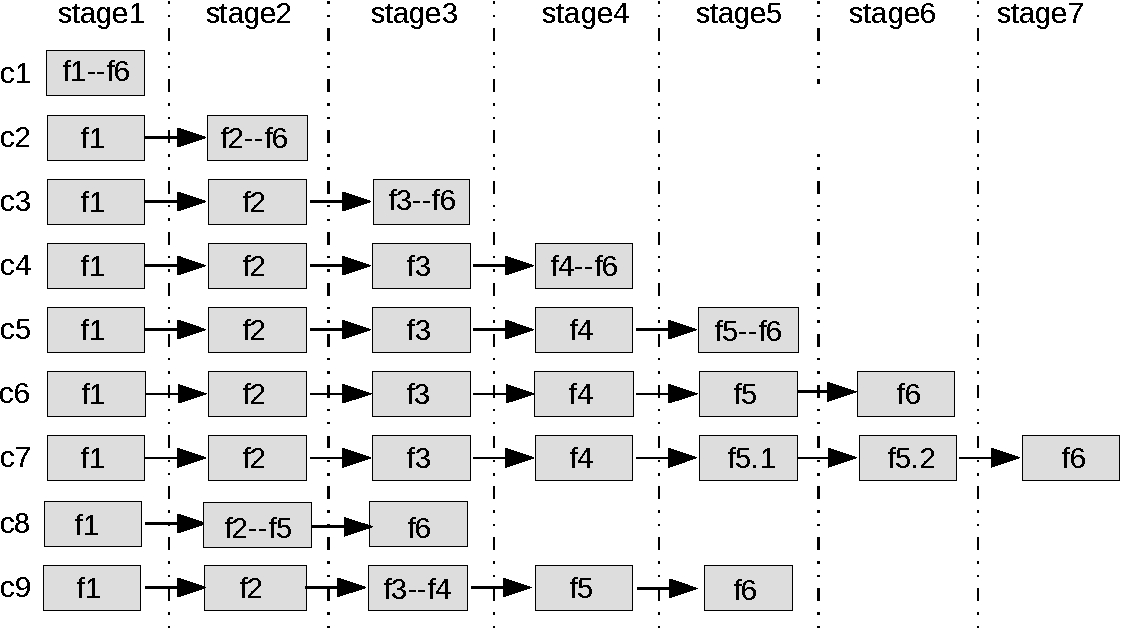
\includegraphics[width=0.95\linewidth]{pipeline-config}}
    \caption{Pipeline configurations with various combinations.}
\label{fig:pipeline-config}
\end{figure}

\begin{figure}
\center{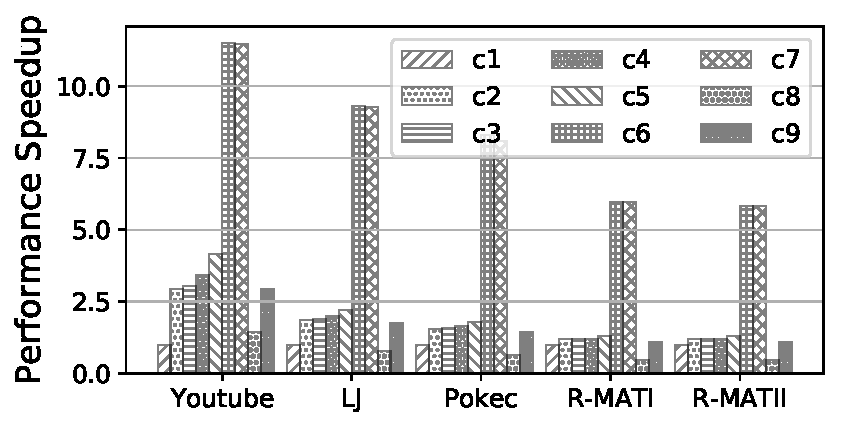
\includegraphics[width=0.95\linewidth]{pipeline-performance}}
    \caption{Performance speedup over a baseline design c1 which 
    is a best effort HLS implementation based on the native nested loop.}
\label{fig:pipeline-performance}
\end{figure}

\subsection{Redundancy removal analysis}
There are large amount of redundant vertices in the frontier neighbors which 
are the major random memory access in BFS as analyzed in Sec \ref{sec:observation}. 
To squeeze the redundancy in the output stream of f4, we create a hash table based 
filter as presented in Section \ref{sec:bfs-opt} and insert it between f4 and f5. 
The hash table size affects both the redundancy removal rate and the resource consumption,
so it must be set properly.

To decide the hash table size, we firstly analyze the correlation 
between the hash table size and the redundancy removal rate with 
fast software emulation. Figure \ref{fig:hash-redundancy} shows the 
redundancy removal rate of different size of hash tables.  Basically larger hash table 
can improve the redundancy removal rate in general, but the improvement gets marginal 
when the hash table size reaches a certain tipping point. Thus the tipping point will be 
an optimized hash table setup. In this work, the tipping point is set to be the hash table size 
when hash hit rate improvement is less than 10\% given double hash table capacity.   
With this metric, the final hash table setup is given in Table \ref{tab:hash-size}.

\begin{figure}
\center{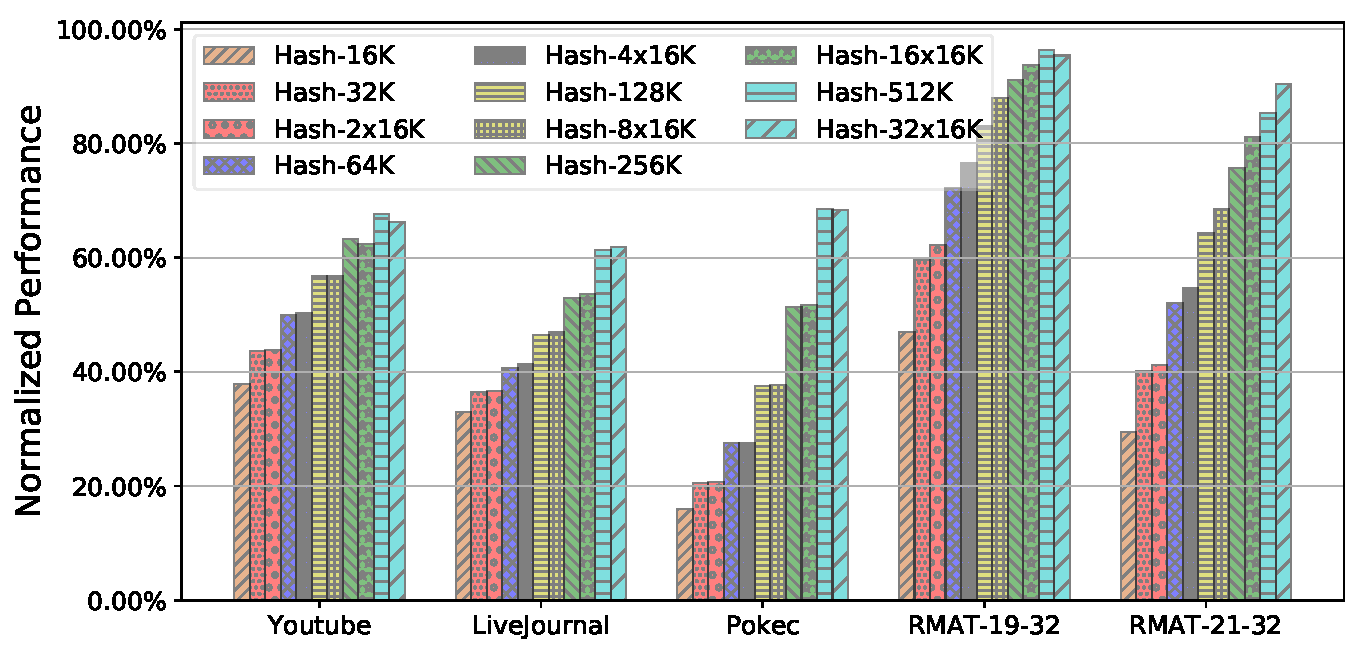
\includegraphics[width=0.95\linewidth]{hash-redundancy}}
    \caption{Redundancy neighbor vertices removal rate with the hash table based filters. 
    The redundancy removal rate is sensitive to the hash table size.}
\label{fig:hash-redundancy}
\end{figure}

\begin{table}
    \centering
  \caption{Hash table size setup}
  \label{tab:hash-size}
  \begin{tabular}{cccccc}
    \toprule
      benchmark & Youtube & LJ & Pokec & R-MAT\uppercase\expandafter{\romannumeral1} 
      & R-MAT\uppercase\expandafter{\romannumeral2} \\
    \midrule
      size (K entries) & 256 & 2048 & 1024 & 512 & 1024 \\
      %size (K entries) & 256 & 2048 & 1024 & 512 & 1024 \\
  \bottomrule
\end{tabular}
\end{table}

\subsection{Cache and prefetch optimization}
In order to take advantage of the memory access locality, 
we develop specific cache and prefetch structures 
for the different processing functions respectively. 
As described in Section \ref{sec:bfs-opt}, we have 
prefetch buffers in S3 and S4 for reading CSR 
and cache structures for random \textit{depth} reading 
and writing in f5 
and f6 respectively. 

Similar to the hash table size setup, we decide the 
prefetch buffer size and cache size through software emulation 
based hit rate analysis. Figure \ref{fig:cache-hit} shows the correlation 
between the prefetch buffer / cache size and the resulting 
hit rate. According to the experiment in the figure,  
the influence of the prefetch buffer varies slightly on different 
graph benchmark and 64B prefetch size achieves satisfactory 
hit rate. 64B is also the optimized internal bus data width 
and a single read operation completes the prefetch simplifying the 
II optimization. With the combined reasons, we choose 64B as the 
prefetch buffer size for all the different graphs.

\begin{table}
    \centering
  \caption{Cache size setup}
  \label{tab:hash-size}
  \begin{tabular}{cccccc}
    \toprule
      benchmark & Youtube & LJ & Pokec & R-MAT\uppercase\expandafter{\romannumeral1}
      & R-MAT\uppercase\expandafter{\romannumeral2} \\
    \midrule
      size (K entries) & 16 & 64 & 16 & 8 & 32 \\
  \bottomrule
\end{tabular}
\end{table}

\begin{figure}
\center{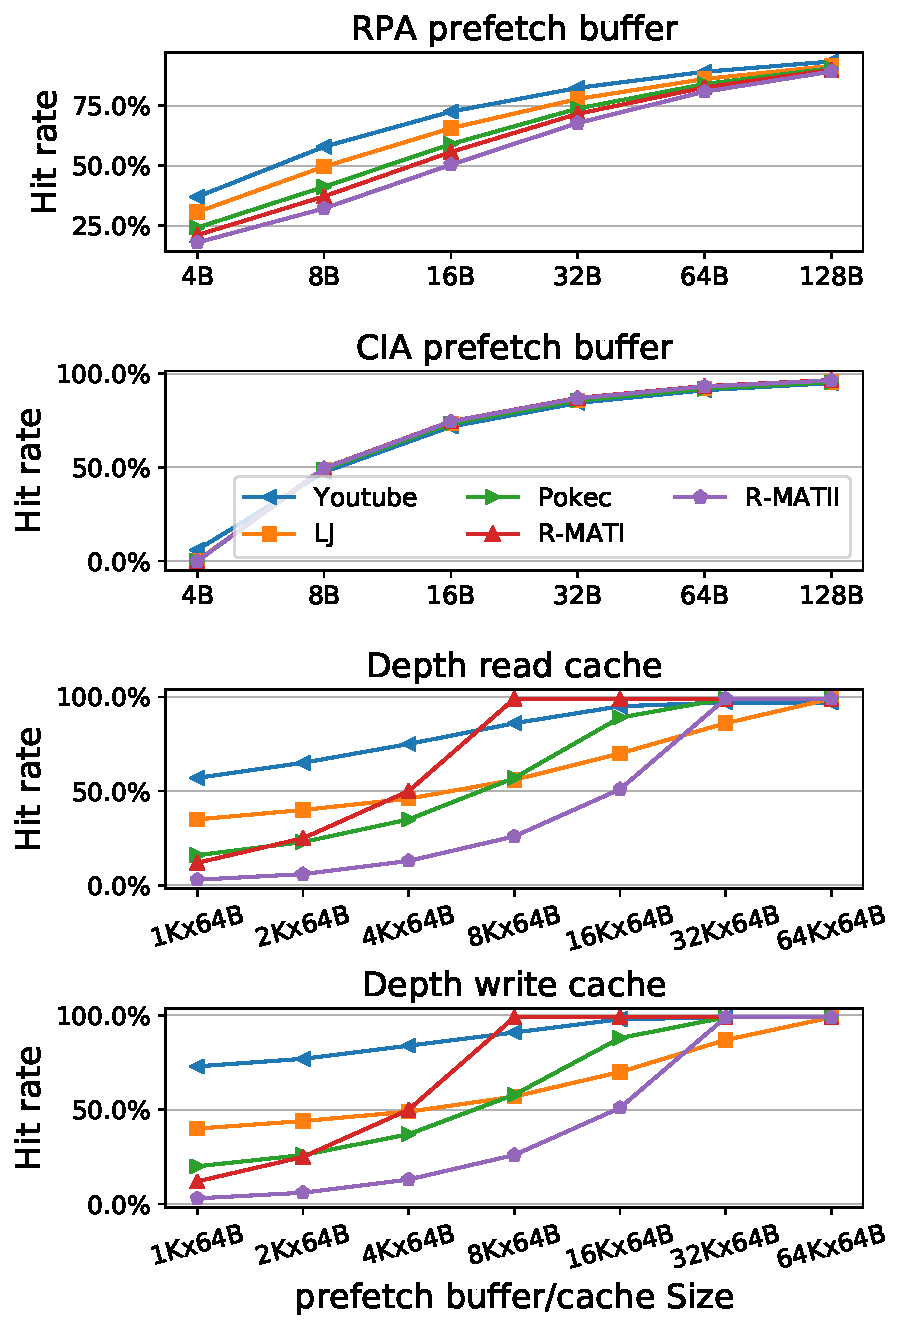
\includegraphics[width=0.95\linewidth]{cache-hit}}
    \caption{Cache and pre-fetch configurations have significant influence on the cache hit rate.
    The influence varies on different graph data set, but the trend is similar.}
\label{fig:cache-hit}
\end{figure}

The cache size influence varies on different graphs. According to the experiments 
shown in Figure \ref{fig:cache-hit}, we find that R-MAT\uppercase\expandafter{\romannumeral1} 
reaches nearly optimal hit rate when the cache size is 8Kx64B i.e. 8K entries with 64B cache line.
For the Youtube and Pokec graphs, cache hit rate is satisfactory when the cache size goes up to 
16Kx64B. Nevertheless, there are still clear hit rate improvement when the cache size increases from 
16Kx64B to 32Kx64B. Particularly, it seems there is still space for cache hit rate 
improvement on the Live Journal graph. In this work, we set the cache size limit to be 32Kx64B for 
better timing as well as fulfilling the resource constraints.

\subsection{Data path duplication optimization}
Data path duplication is a simple yet efficient way to improve the memory 
bandwidth utilization as well as overall BFS accelerator performance. However, 
the SDAccel allows at most 16 global memory ports in a hardware thread while 
the amount of global memory ports increases when the data path is duplicated.
Using the data path duplication strategy proposed in Sec \ref{sec:bfs-opt}, we
can implement at most 4 lanes of data paths. Moreover, the cache size and hash 
table size must also be adjusted accordingly to fit for the block ram resource 
constraint while replicating the data paths. The detailed configuration of the 
data path duplication based design is shown in Table \ref{tab:duplication-config}.
Copared to the expected optimized setup, the final setup is not optimal due to the 
relatively small amount of on chip block ram budget on Alpha Data.
While prefetch buffer remains the same for all the configurations, they 
are not listed in the table to save space.

% \usepackage{multirow}
\begin{table}[]
    \centering
    \label{tab:duplication-config}
    \caption{Data path duplication setup}
    \label{my-label}
    \begin{tabular}{c|c|ccccc}
        \toprule
        %\hline
        \multicolumn{2}{c|}{benchmark} & Youtube & LJ & Pokec 
        & R-MAT\uppercase\expandafter{\romannumeral1} & R-MAT\uppercase\expandafter{\romannumeral2} \\ 
        \midrule
        \multirow{2}{*}{2 lanes}  & hash table  & 256K & 512K & 1024K & 512K & 1024K \\ \cline{2-7} 
                           & read cache & 16K & 16K & 16K & 8K & 16K \\ \cline{2-7}
                           & write cache & 16K & 16K & 16K & 8K & 16K \\ \hline
        \multirow{2}{*}{4 lanes}  & hash table  & 256K & 1024K & 1024K & 512K & 1024K \\ \cline{2-7} 
                           & read cache & 8K & 8K & 8K & 8K & 8K \\ \cline{2-7}
                           & write cache & 16K & 16K & 16K & 8K & 16K \\ \hline
    \end{tabular}
\end{table}

\subsection{Optimization implementation evaluation}
After tuning the design parameters gradually, we evaluate the 
performance of the BFS accelerator with the optimization techniques based on 
the hardware implementation. Basically we start from the baseline design and 
add the optimizations including pipelining, hash redundancy removal, 
prefetching, caching and data path duplication in order. The performace improvement 
with these optimizations can be found in Figure \ref{fig:opt-performance}. 
It can be found that the performance of the BFS accelerator improves 
significantly when an optimization technique is applied. According to the figure,
pipeling and data path duplication enhance the performance most 
significantly. The performance improvement brought by the hash table based filtering 
seems to be trivial, but it actually boosts the performance by over 20\% on average. 

\begin{figure}
\center{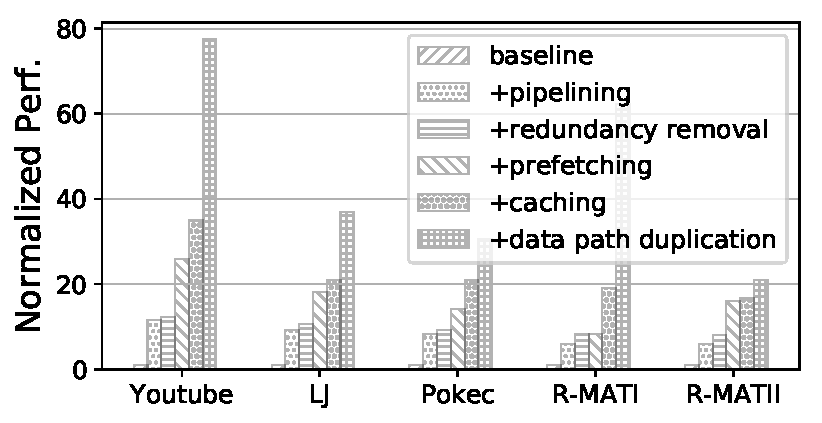
\includegraphics[width=0.95\linewidth]{opt-performance}}
    \caption{BFS accelerator optimization techqniue evaluation. The performance on 
    all the graphs improves when more optimizations are added to the design, though 
    the performance improvement varies on different graphs and optimizaion 
    techniques.}
\label{fig:opt-performance}
\end{figure}

\section{Conclusions} \label{sec:conclusion}
Handcrafted HDL based BFS accelerators usually suffer high portability and maintenance cost 
as well as ease of use problem despite the relatively 
good performance. HLS based BFS accelerator can greatly alleviate these problems, but it is 
difficult to achieve satisfactory performance due to the inherent irregular memory access and 
complex nested loop structure. In this work, we stream the basic BFS algorithm and implement a 
highly pipelined BFS accelerator using C/C++ HLS on state-of-art Xilinx SDAccel platform. In addition, 
we further improve the performance of the HLS design with a series of optimizations such as 
redundancy removal, prefetching, caching and data path duplication. According to the experiments on 
a representative graph benchmark, the resulting HLS based BFS accelerator achieves up to 70X speedup 
compared to a baseline HLS design with best-effort HLS pragma optimization. When compared to the 
existing HDL based BFS accelerators on similar FPGA cards, the proposed HLS based BFS accelerator 
gets around 35\% of the MTEPS, but it preserves the nice software-like features including 
portability and ease of use and maintenance, and achieves higher per bandwidth MTEPS mostly 
because of the graph specific optimization techniques. 

